\documentclass[11pt]{article}
\usepackage{graphicx}
\usepackage{geometry}
\usepackage{fancyhdr}
\usepackage{setspace}
\usepackage{indentfirst}
\usepackage{gensymb}

\geometry{a4paper, margin=1in}
\pagenumbering{roman}
\doublespacing


\fancyhf{}
\fancyhead[RO,LE]{CIVIC}
\fancyfoot[C]{\thepage}
\pagestyle{fancy}

\begin{document}

\thispagestyle{empty}
\begin{titlepage}
    \begin{center}
        \textbf{\Large CIVIC (Central Intelligence Virtualization Instruction Cluster)} \\[1cm]
        A capstone project report submitted in partial fulfillment of the requirements for the degree of \\[1cm]
        \textbf{\Large Masters of Engineering} \\[1cm]
        In the Department of Computer Science Graduate Program, \\
        College of Engineering \& Applied Science \\[1cm]
        04/11/2025 \\[1cm]
        Margeson, Jack
    \end{center}
\end{titlepage}

\setcounter{page}{2}
\section{Abstract}

Distributed computing is a design methodology that enables digital storage and data processing to be completed across multiple devices, often on separate networks. CIVIC (Central Intelligence Virtualization Instruction Cluster) allows organizations (labs, campuses, businesses, etc.) to deploy their own instance of a cooperative computational system. CIVIC’s platform streamlines program development for organizations by leveraging virtualization technologies, and the user-friendly and flexible workflow allows participants to easily volunteer computational resources to CIVIC instances.

The overall goal of this project is to address the limitations of current volunteer distributed computing programs and open new possibilities for research and development. Unlike existing frameworks that require specific programming languages or hardware architectures when writing applications, CIVIC provides a flexible language and architecture-independent design.

Researchers can deploy their existing code to a CIVIC instance with minimal changes, while participants can easily contribute computational resources. This is achieved through the creation of models, a set of instructions that can be used by client machines to create virtualizations. These virtualizations, referred to as citizens, are worker containers capable of receiving fractions of input data and executing code to generate output. Each fraction of data generated by the server is called a duty, and each duty can be assigned to one or more citizens depending on the result verification needs of the project.

The CIVIC Server manages model distribution and communication with citizens, as well as processing, validating, and assimilating incoming duty results---ensuring efficient and scalable distributed computing by minimizing required human interaction from both organization and participant perspectives.

\section*{Acknowledgements}

I would like to extend my thanks to my faculty advisor, Dr.\ William Hawkins III, for his guidance and encouragement throughout the development of this capstone project. I would also like to thank my coworkers from co-op rotations at London Computer Systems, 84.51\degree, and Siemens for helping me improve my skills with full stack development and learn best practices in an industry setting. Finally, I would like to thank my family and friends for their support and confidence in me throughout my academic career.

\section{Introduction}

In the field of distributed computing, one interesting utilization of the concept is volunteer computing software. Applications and services that fall under this category, including SETI@home, XtremWeb, and BOINC~\cite{Mengistu2020}, allow users to donate their idle computing resources to scientific research projects. These projects typically require large amounts of computational power to process data, and volunteer computing allows researchers to leverage the collective power of many individual computers. For example, one of the more popular volunteer computing applications, Folding@home, is used to simulate protein folding to contribute to scientific research through the study of diseases such as COVID-19 and Alzheimer's~\cite{Voelz2023}. The protein folding process is a complex mathematical simulation that requires significant computational resources to run. For problems like these, volunteer computing is a useful technology to leverage the computing power of several machines to independently work on fractions of the problem. Utilizing volunteer computing in a scenario like this reduces the overall time that it would take one machine to complete the task, and allows researchers to run simulations on a larger scale than would be possible with a single machine.

However, there are limitations to some of the existing volunteer computing frameworks. For example, we can examine BOINC, the the Berkley Open Infrastructure for Network Computing~\cite{Anderson2020}. BOINC is a framework that enables researchers to create their own volunteer computing projects and allows volunteers to donate computational resources to any of these projects by downloading the client and selecting from a list of available causes. One of the big issues when it comes to creating a research project on BOINC is the fact that programs that are to be distributed to volunteers must be packaged in a very specific way. The BOINC framework provides three options for application developers~\cite{boincAppsIntro}:

\begin{itemize}
    \item Native applications, in which the program must be written in a language that supports the official BOINC API and compiled for a target architecture.
    \item Wrapper applications, in which a program is written in a language that does not support the official BOINC API but can be run as a sub-process of a wrapper application that handles input and output.
    \item Virtual applications, in which a program is run in a virtual machine that is managed by the BOINC framework through external scripts and programs such as VirtualBox.
\end{itemize}

Each of these options have their own limitations. With native applications, the developer of the program must write in a programming language that either officially supports (C/C++) or unofficially supports (FORTRAN, Python) the BOINC API interface. For both native and wrapper applications, the program that is written must be compiled for a target architecture before distributed to a client. The implication of this is that if a researcher would like to allow participants to contribute to the project, they must first compile any programs written for the project for each architecture that they would like to support, i.e.\ x86 Windows, x86 Linux, ARM Linux, Android, etc. This can be a time consuming process, especially when program changes are made and then must be recompiled for each supported architecture. Additionally, code changes must be made to programs when dealing with certain functionality, such as differences in how system commands and file operations are handled between Windows and Unix based operating systems. The third option, virtual applications, mitigates some of the problems with native and wrapper applications. These types of BOINC applications are able to execute in a virtual machine, which allows the program to be written in any language and run on any architecture. However, this option entails significant additional setup and configuration with an external program, VirtualBox, which can introduce additional complexity, runtime overhead, and download size for volunteers.

These limitations are not exclusive to BOINC---several other volunteer computing frameworks have similar restrictions. In this capstone report, a new alternative to existing volunteer computing frameworks is proposed. CIVIC (Central Intelligence Virtualization Instruction Cluster) is a framework that utilizes virtualization technology to allow researchers to easily create and deploy volunteer computing projects. By utilizing virtualization, CIVIC allows for the development of language and architecture independent applications. In combination with a binary application distributable, researchers can use the framework to parse and create datasets to create models for distribution. Volunteers looking to contribute to research are able to donate their computational resources to a project by creating a `citizen'---a virtual client program that runs in it's own isolated container environment. These citizens automatically download and execute model instructions given from the server with a subset of the input dataset and return the results to the server. The primary goal of CIVIC is to provide a framework that allows easy configuration and deployment of volunteer computing projects for researchers, while also providing a simple and user-friendly experience for volunteers looking to contribute to research. The framework is designed to be flexible and extensible, allowing researchers to easily adapt it to their specific needs.

\section{Methods}

The architecture of the framework can be split into two main components: the server and the client. Together, the server and client implementations comprise the technology stack powering the CIVIC framework. The server component is responsible for managing the distribution of models, binaries, duties, and other instructions to connected clients. The client component, or citizen, is a container that receives inputs and commands from the server and returns outputs of executed duties.

Two scripts are provided to facilitate the installation and management of the server and client components---\verb|server_manager.py| and \verb|client.py|. In addition to server installation, the server manager script is also used to create new models for the server to distribute, as well as parsing and generating datasets for those models. The client script is used to create new citizens that connect to the server and execute duties.

To achieve the server-client architecture outlined, several technologies are used. The first of these technologies is Docker, a containerization software that allows for programs to be run in an isolated environment. Docker and the Docker Engine API are used in both the server and client components of CIVIC.\@ The installation of a CIVIC server is handled through the server manager script which integrates with the Docker SDK to build and manage Docker images and containers that power the server.\@ With the use of Docker, the script builds and installs four services: the `internal CIVIC server', a Python Flask middleware application, a PostgreSQL database, and Adminer, an external database management tool. In addition to handling image builds and container management, the installation process also creates volumes (persistent data) on the server machine for database use, as well as a virtual network bridge to facilitate communication between the four services. 

The first of the four services, the internal CIVIC server, is a Python script that is in charge of handling connections with clients, downloading and distributing model files and datasets, and generating duties for clients to execute. The application utilizes \verb|curses|, a Python extension module that enables finer control over terminal interfaces to create a console interface for management. This console can be accessed through the use of the server manager script by attaching to the Docker container. Within the console, the user can execute several commands to facilitate the operations outlined above. 

Python Flask is used to create the second core services of the server, enabling intra-service communication via RESTful API calls. The Flask application contains several endpoints that allow the internal CIVIC server to talk to the PostgreSQL database. This middleware directly connects to the PostgreSQL database through the use of the \verb|psycopg2| Python library, which enables SQL queries to be execute when connected to remote databases. Since all communication between client and server is done through the internal CIVIC server, clients do not directly interact with the Flask application. 

PostgreSQL, the database software that makes up the third core service, is used to store information about models, duties, and clients. It is queried through use of RESTful API endpoints exposed in the Flask service to retrieve and store information about the state of the CIVIC network. Several tables are created on installation of the server---and two additional tables are created upon the addition of a new model to store both the model's dataset and the results of duties executed by clients pertaining to that model. 

The final core service, Adminer, is an external database management tool that allows for the viewing and editing of the PostgreSQL database. Adminer is a web-based application that can be accessed through a web browser on the server machine. The tool is used to view the contents of the database, as well as to make changes to the database if necessary. Adminer is not required for the operation of the CIVIC server, but is included as a convenience for users who may want to view the contents of the database without needing to use the command line.

Combined, these four services create a server that is capable of managing the distribution of models and duties to clients and storing results for future analysis. The server is designed to be scalable, allowing for the addition of new clients and models as needed. The server is also designed to be fault-tolerant, with the ability to recover from crashes and other failures by utilizing the persistent data stored in the PostgreSQL database volume and Docker monitoring and container restart capabilities.

On the client side, the Docker SDK is used once again with the \verb|client.py| script to build a single Docker image---the \verb|internal_client| service, which, when run as a container, acts as a citizen in the CIVIC network. The citizen containers run on Alpine Linux, a lightweight and simple Linux distribution often used in combination with Docker due to the operating system's small file size and resource overhead. This container is `dumb' in the sense that when created, it no longer needs to communicate with the client machine that initializes it. Citizen containers retry their connection to the IP and port provided during creation until they are able to connect. Once connected, citizens will wait for instructions given by the central server. When prompted, the citizen will download model binaries and datasets from the server, execute the model with the given dataset slice, and return the results to the server. The citizen will then wait for the next instruction from the server, repeating the process until the server has no more duties to distribute. This process is repeated for each citizen in the network, allowing for the distributed execution of models across multiple instances of citizens on the same machine, citizens on multiple machines, and citizens on multiple external networks. 

\section{Results}

The results of the CIVIC framework are promising. The server component is able to successfully manage multiple citizens connected from multiple different machines and distribute instructions, models, and datasets to those citizens. As stated previously, two Python scripts, \verb|server_manager.py| and \verb|client.py|, have been designed with simple terminal console-like interfaces to equip both researchers and volunteers with easy to understand tools to manage the server and client components respectively. These management scripts are able to run on any machine that supports Python 3.13 or higher and Docker, allowing the setup for any user to be performed with straightforward and minimal requirements.

\begin{figure}[h]
    \centering
    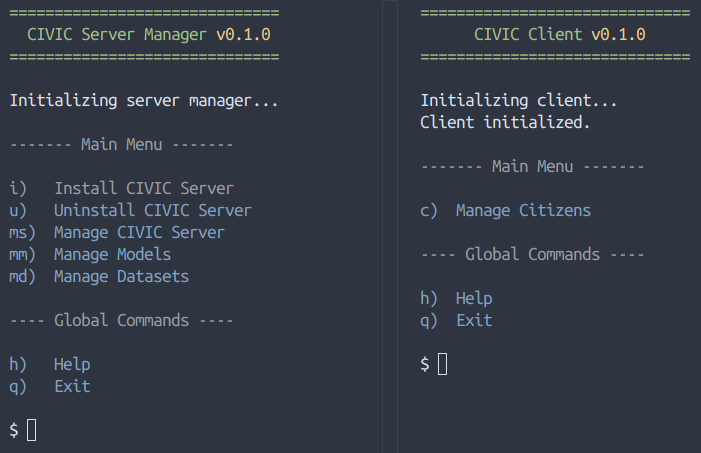
\includegraphics[width=0.7\textwidth]{./figures/terminals.png}
    \caption{\small The \texttt{server\_manager.py} and \texttt{client.py} scripts running in separate terminal windows.}\label{fig:terminals}
\end{figure}

In addition to the creation of the CIVIC, this project also contains a proof of concept model that demonstrates the capabilities of the framework. Included in the project's code repository is a simple model called \verb|Alphabet|. The \verb|Alphabet| model is a simple program that takes a single letter as input and returns the next letter in the alphabet as output, followed by the burning of CPU cycles for a short amount of time to simulate a heavier workload, which is typical in demonstrations of distributed computing. The model binary is written in C, compiled for Linux x86 architecture, and designed to be simple and easy to understand, making it a good starting point for researchers looking to create their own models for the CIVIC framework. As illustrated in Figure~\ref{fig:internal_server}, the model is able to successfully run on multiple citizens connected to the server, with each citizen executing a different duty and returning the results to the server. 

\begin{figure}[h]
    \centering
    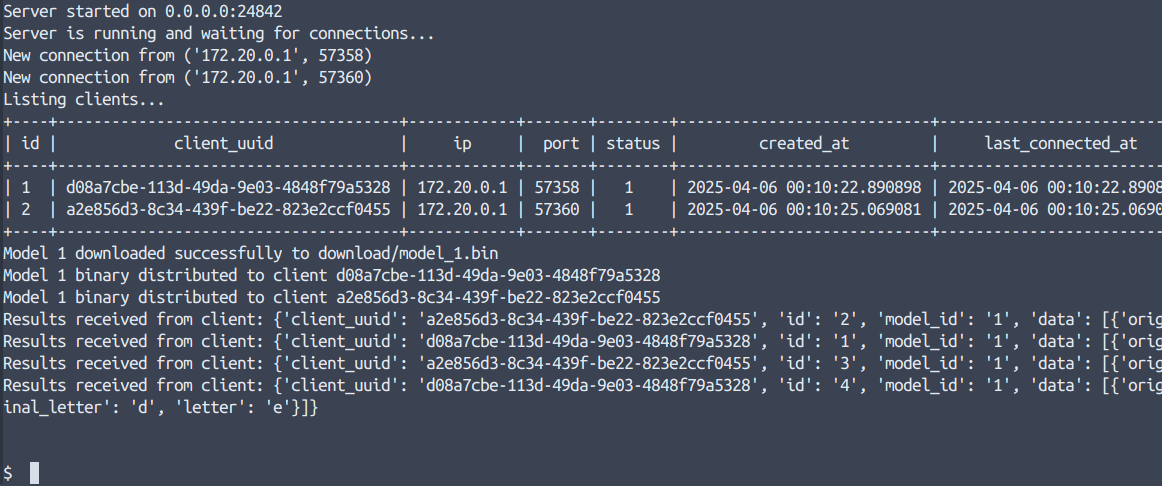
\includegraphics[width=0.9\textwidth]{./figures/internal_server.png}
    \caption{\small The internal server console interface creating duties from the Alphabet model.}\label{fig:internal_server}
\end{figure}

The results of the duties are stored in the PostgreSQL database, which can be viewed through Adminer or through the console interface of the server manager script. A slice of results are shown in Figure~\ref{fig:alphabet_1}. These results show that the model is able to successfully execute on multiple citizens, with each citizen returning a different result based on the fraction of input data provided with each duty. The results are stored in the database, allowing for easy access and analysis of the data generated by the model. Further analysis of the results can be performed using SQL queries or through the use of external data analysis tools.

\begin{figure}[h]
    \centering
    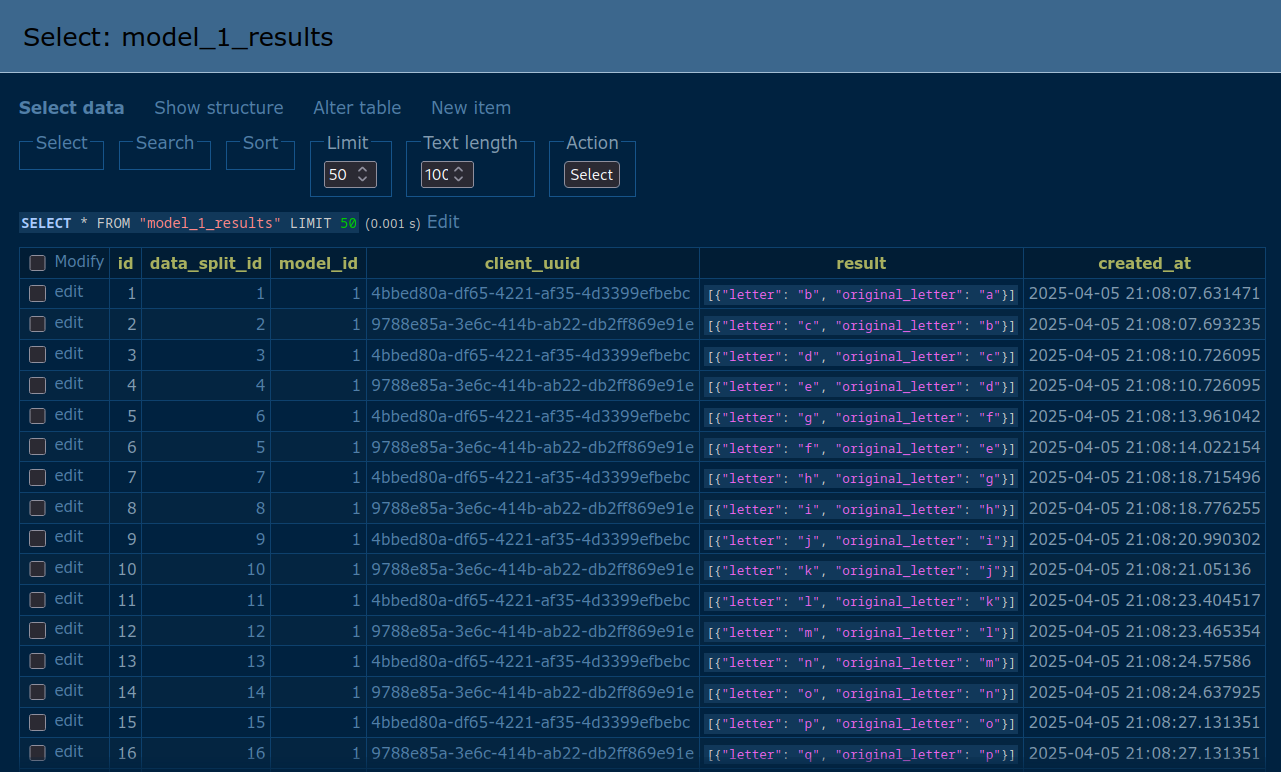
\includegraphics[width=0.8\textwidth]{./figures/alphabet.png}
    \caption{\small The results of the Alphabet model running on multiple citizens connected to the server.}\label{fig:alphabet_1}
\end{figure}

\newpage

\section{Discussion}

While the CIVIC framework provides a functional alternative to existing volunteer computing frameworks by incorporating new features like virtualization, there are several future improvements that could be made to the system. In this section of the report, a select few of these potential improvements will be discussed. 

The first of these improvements is the addition of a web-based interface for the server. Currently, the server is managed through a console interface that is accessed through the server manager script. While this interface is functional, it may be difficult to use for users who are not familiar with command line interfaces. A web-based interface would allow users to manage the server through a web browser, making it more accessible to a wider audience. This could be achieved by creating a web application that communicates with the Flask middleware and PostgreSQL database to provide options for managing models, duties, and clients via the browser. In addition, a web-based interface could allow for the implementation of several data visualization techniques such as the D3 JavaScript library to provide researchers an easier way to conceptualize the results of the work done without exporting the data to a separate program.

One other potential improvement would be support for more specific workflows. Currently, the CIVIC framework is designed to be flexible enough to run the majority of volunteer computing projects that a researcher may be interested in creating. However, there are several specific workflows in the field of distributed computing that require more tailored functionality. For examples, we turn to other volunteer computing frameworks such as Mining@home~\cite{Lucchese2010}. The Mining@home framework has been specifically designed to facilitate data mining problems, such as itemset mining and clustering. This functionality was achieved through the introduction of peer-to-peer communication between clients (referred to as miner nodes) and new server-side features tailored to the distribution of data mining tasks, as the traditional server-client architecture is not well suited for these types of problems. The addition of features like the ones presented in Mining@home and other pre-existing specialized frameworks would allow for the CIVIC framework to be used in a wider variety of research projects.

Finally, the addition of a more robust error handling and caching system could be of use in the CIVIC framework to better mitigate data and work losses from client crashes and other failures. The framework is currently designed to be fault-tolerant, but there are still several edge cases that could be improved upon. For example, if a citizen crashes while executing a duty, the server will not be able to recover the results of that duty. The introduction of a caching system, as elaborated upon in the article `A Scalable Framework for Wireless Distributed Computing'~\cite{Li2017}, has several advantages when implemented into a distributed computing platform. Alongside the ability to better handle crashing from the client side by caching results periodically, a caching system would additionally allow for pre-fetch content to be distributed between multiple clients on a separate network, reducing the amount of data that needs to be sent from the central server.

\section{Conclusion}

In conclusion, the CIVIC framework provides a functional and flexible alternative to existing volunteer computing frameworks. By utilizing virtualization technology, CIVIC allows researchers to create and deploy volunteer computing projects with minimal effort while maintaining user-friendliness and accessability. The proof of concept model demonstrates the capabilities of the framework and shows that it is able to successfully manage multiple citizens connected from multiple different machines and distribute models, binaries, and duties to those citizens. While there are several potential improvements that could be made to the framework, the current implementation provides a solid foundation for future development. It is hoped that the CIVIC framework will be able to contribute to the field of distributed computing and enable researchers to leverage the power of volunteer computing in their work.


\newpage
\thispagestyle{empty}
\nocite{*} % Lists entire bibliography regardless of citation
\renewcommand{\refname}{Bibliography} % Change References -> Bibliography
\bibliographystyle{ieeetr}
\bibliography{civic} 

\end{document}
